\documentclass[aspectratio=169,10pt]{beamer}
\usepackage[utf8]{inputenc}
\usepackage[T1]{fontenc}
\usepackage{lmodern,amsmath,amssymb,booktabs,array,graphicx}
\usepackage{beamerthemeicshm}
\newcommand{\structmiou}{\mathrm{mIoU}_{\mathrm{struct}}}
% Internal traceability only. Source arguments remain in presentation.tex but
% are intentionally omitted from the rendered conference slides.
\newcommand{\source}[1]{}
\newcommand{\tightitems}{\setlength{\itemsep}{0.32em}\setlength{\parskip}{0pt}}

\graphicspath{{../figures/}}
\title{Multi-View Semantic 3D Gaussian Splatting for\\Component-Aware Bridge Reconstruction from UAV Imagery}
\subtitle{Rendering bridge appearance and structural components from arbitrary viewpoints}
\author{Quoc-Bao Ta\inst{1} \and Trung Ha Nguyen\inst{2} \and Thai Ha Dang\inst{3}}
\institute{\inst{1} Department of Civil Engineering, University of Texas Rio Grande Valley, Edinburg, TX, USA\\\inst{2} Jisan Construction Co., Ltd., Busan, South Korea\\\inst{3} Department of Electrical Engineering, University of North Texas, Denton, TX, USA}
\date{IC-SHM Competition -- Project 2\\September 2026}
\begin{document}

\begin{frame}[plain]
\vspace{0.15cm}\begin{beamercolorbox}[wd=\textwidth,sep=.32cm,center,rounded=true,shadow=true]{frametitle}{\usebeamerfont{title}\inserttitle\par}\vspace{.15cm}{\usebeamerfont{subtitle}\insertsubtitle}\end{beamercolorbox}
\vspace{.42cm}\begin{center}{\usebeamerfont{author}\insertauthor}\par\vspace{.18cm}{\usebeamerfont{institute}\insertinstitute}\par\vspace{.25cm}{\normalsize\insertdate}\end{center}
\vfill\hfill{\tiny 1\,/\,\inserttotalframenumber}
\end{frame}

\section{Task and data}
\begin{frame}{Competition task}
\begin{itemize}\tightitems
\item IC-SHM 2026 Project 2 asks for a renderable semantic reconstruction of one suspension bridge from posed UAV imagery.
\item A query camera pose must produce an RGB image and a five-class map: background, deck, stay cable, tower, and foundation.
\item The organizers use PSNR, SSIM, LPIPS, and semantic mIoU on an unreleased blind set. Our results use a separate local 30-view holdout \textup{[1]}.
\item The target is a component-aware scene representation. Damage detection, deformation measurement, and survey-grade geometry are outside this evaluation.
\end{itemize}
\begin{block}{Objective}Learn one 3D representation that renders aligned appearance and component labels from supplied or constructed viewpoints.\end{block}
\source{IC-SHM 2026 Project 2 brief; DRAFT.md Sections 1 and 3.1.}
\end{frame}

\begin{frame}{Released data and required output}
\begin{columns}[T,onlytextwidth]\column{.52\textwidth}
\begin{itemize}\tightitems
\item 400 UAV photographs at $1320\times989$ pixels.
\item 300 images contain polygons for four bridge components and background.
\item 100 images contain RGB only. Our pipeline generates pseudo-labels so these views can provide semantic supervision.
\item SIMPLE\_RADIAL calibration, camera poses, and COLMAP feature tracks are supplied, but no precomputed 3D points.
\end{itemize}
\column{.45\textwidth}
\begin{block}{Renderer interface}Input: rotation, translation, intrinsics, image size.\\[.3em]Output: RGB $\hat I$ and class map $\hat M\in\{0,\ldots,4\}^{H\times W}$.\end{block}
\begin{block}{Local partition}240 labeled train + 30 labeled validation + 30 labeled test; 100 unlabeled views remain separate.\end{block}
\end{columns}
\source{DRAFT.md Sections 3.1, 3.6, and 4.1.}
\end{frame}

\begin{frame}{Related methods and our design choice}
\footnotesize\begin{tabular}{>{\raggedright\arraybackslash}p{.18\textwidth}>{\raggedright\arraybackslash}p{.25\textwidth}>{\raggedright\arraybackslash}p{.47\textwidth}}\toprule
Family & Capability & Choice for this task\\\midrule
NeRF & Implicit novel-view synthesis & Useful precedent, but no explicit primitive for a bridge-component label.\\
3D Gaussian Splatting \textup{[3]} & Explicit primitives and differentiable rasterization & Store RGB and five semantic logits on every Gaussian.\\
Semantic/feature scene models \textup{[4,5]} & Render labels or learned features & Optimize fixed-class logits directly instead of open-vocabulary features.\\
SegFormer \textup{[6]} & Efficient multi-scale segmentation & Generate pseudo-labels for the 100 unlabeled views.\\
COLMAP geometry & Posed multi-view tracks & Triangulate after excluding test observations.\\\bottomrule
\end{tabular}
\vspace{.3em}The contribution is a task-specific integration for UAV bridge data, not a claim that semantic attribute rendering is new.
\source{DRAFT.md Section 2; Kerbl et al. (2023); Xie et al. (2021).}
\end{frame}

\section{Method}
\begin{frame}{Proposed pipeline}
\begin{columns}[c,onlytextwidth]
\column{.72\textwidth}
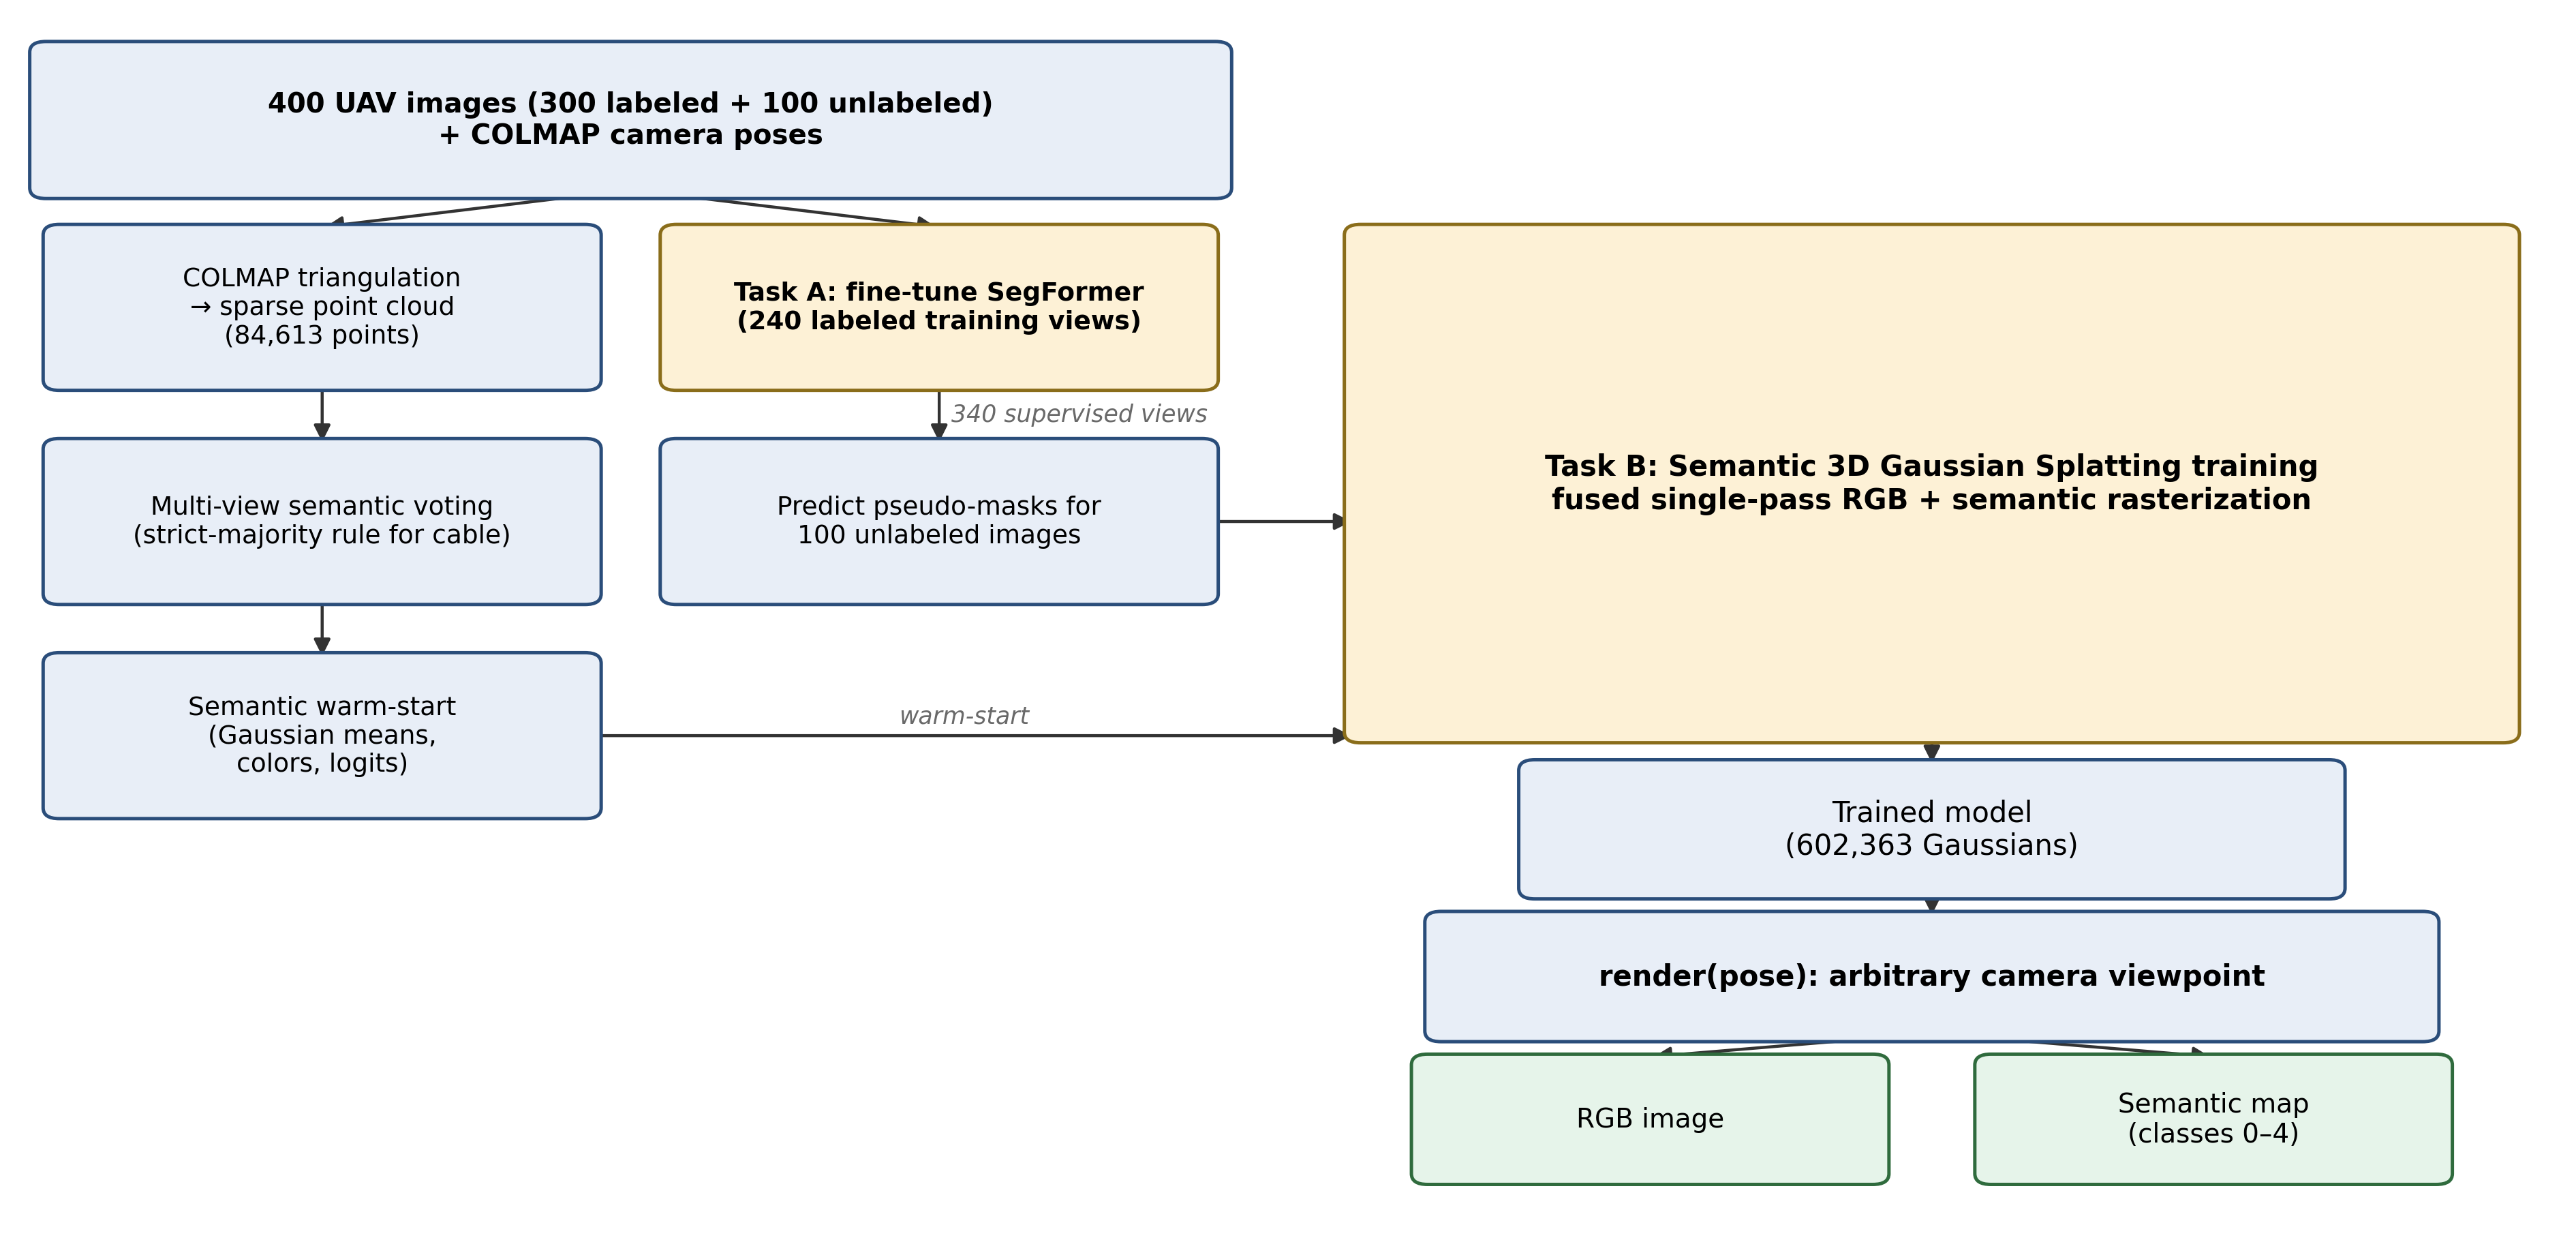
\includegraphics[width=\textwidth,height=.80\textheight,keepaspectratio]{fig1_pipeline.png}
\column{.25\textwidth}
\small
\begin{itemize}\tightitems
\item \textbf{Task A} trains on 240 views, selects on 30, and labels 100 unlabeled views.
\item \textbf{Task B} jointly optimizes RGB and semantics from 370 supervised views.
\item One trained scene renders an RGB image and a five-class map from a query pose.
\end{itemize}
\end{columns}
\source{DRAFT.md Figure 1 and Section 3.}
\end{frame}

\begin{frame}{Data split and test isolation}
\begin{columns}[T,onlytextwidth]\column{.56\textwidth}
\begin{itemize}\tightitems
\item Every tenth labeled image forms the 30-view test split.
\item Every ninth image among the remaining 270 forms Task A's 30-view validation split; 240 images train SegFormer.
\item Task B uses 270 non-test labeled views and 100 pseudo-labeled views.
\item Test images contribute to no Task A training or selection and no Task B model-building step.
\end{itemize}
\column{.41\textwidth}
\begin{block}{Excluded test information}Task B losses\\semantic voting\\sparse triangulation\\observed-color initialization\end{block}
\begin{alertblock}{Scope}Organizer-supplied calibration and poses are retained, so evaluation conditions on supplied camera geometry.\end{alertblock}
\end{columns}
\source{DRAFT.md Section 3.6.}
\end{frame}

\begin{frame}{Camera geometry and sparse initialization}
\begin{itemize}\tightitems
\item Removing test observations leaves 86,319 tracks from the 370-image training pool.
\item LO-RANSAC uses a $2^{\circ}$ angular threshold, a $0.5^{\circ}$ minimum triangulation angle, and cheirality checks.
\item Triangulation produces 84,086 points with 0.49-pixel mean reprojection error; a quartile-distance filter leaves 82,518 initial Gaussians.
\item Track-coordinate color sampling and semantic voting use original images. Task B images and masks are undistorted into the same pinhole coordinates.
\item Nearest-neighbor mask remapping preserves discrete class IDs.
\end{itemize}
\begin{block}{Coordinate rule}Original space: feature tracks, sampled colors, votes. Undistorted space: Task B rendering, losses, and evaluation.\end{block}
\source{DRAFT.md Section 3.2.}
\end{frame}

\begin{frame}{Task A: SegFormer pseudo-labeling}
\begin{center}
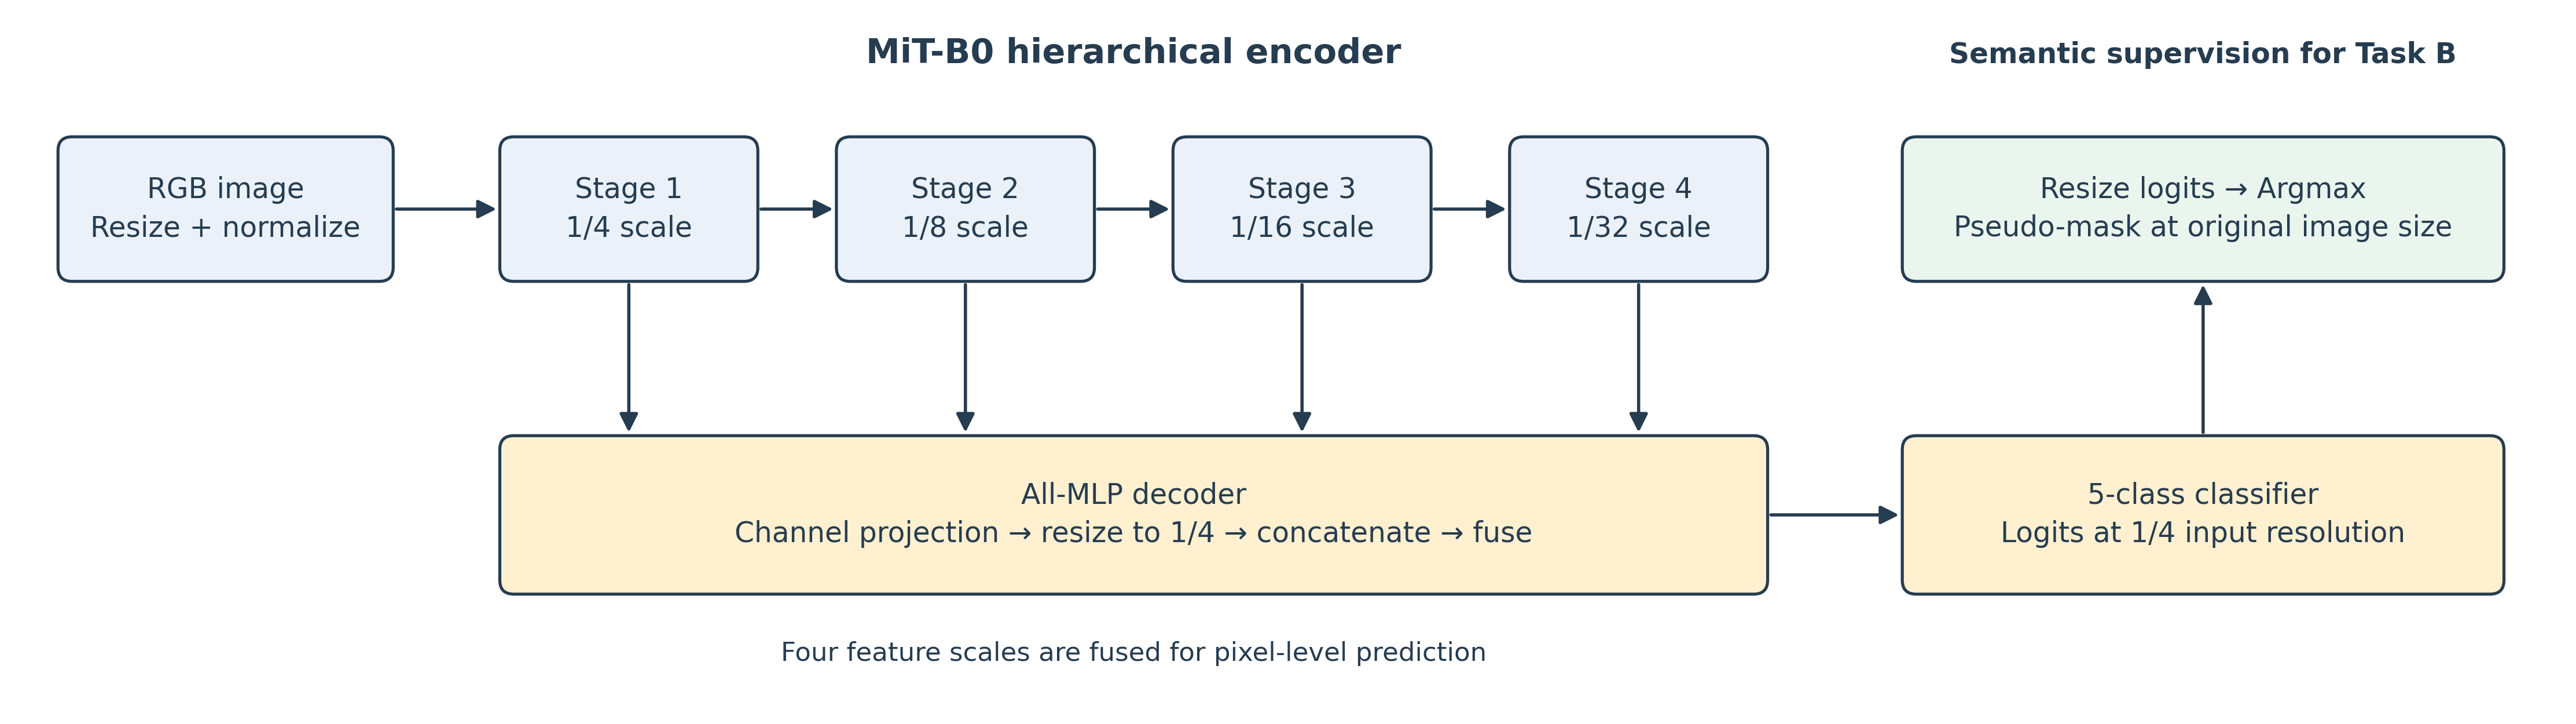
\includegraphics[width=.90\textwidth,height=.56\textheight,keepaspectratio]{fig2_segformer_architecture.png}
\end{center}
\vspace{-.3em}
\begin{itemize}\tightitems
\item The MiT-B0 encoder extracts four feature scales; the all-MLP decoder fuses them and predicts five-class logits \textup{[6]}.
\item Training uses 240 labeled images and checkpoint selection uses 30 validation views. The 30 test images never influence Task A.
\item Resizing logits to the original image dimensions followed by argmax generates masks for the 100 unlabeled images.
\end{itemize}
\source{DRAFT.md Section 3.3 and Figure 2.}
\end{frame}

\begin{frame}{Task A protocol and validation result}
\begin{columns}[T,onlytextwidth]\column{.42\textwidth}
\begin{tabular}{lr}\toprule Class & IoU\\\midrule deck&92.80\%\\stay\_cable&89.17\%\\tower&78.20\%\\foundation&66.48\%\\background&98.64\%\\\midrule\textbf{Structural mIoU}&\textbf{81.67\%}\\\bottomrule\end{tabular}
\vspace{.4em}\small 80 epochs, batch 8, AdamW, $512\times384$; best checkpoint at epoch 69.
\column{.55\textwidth}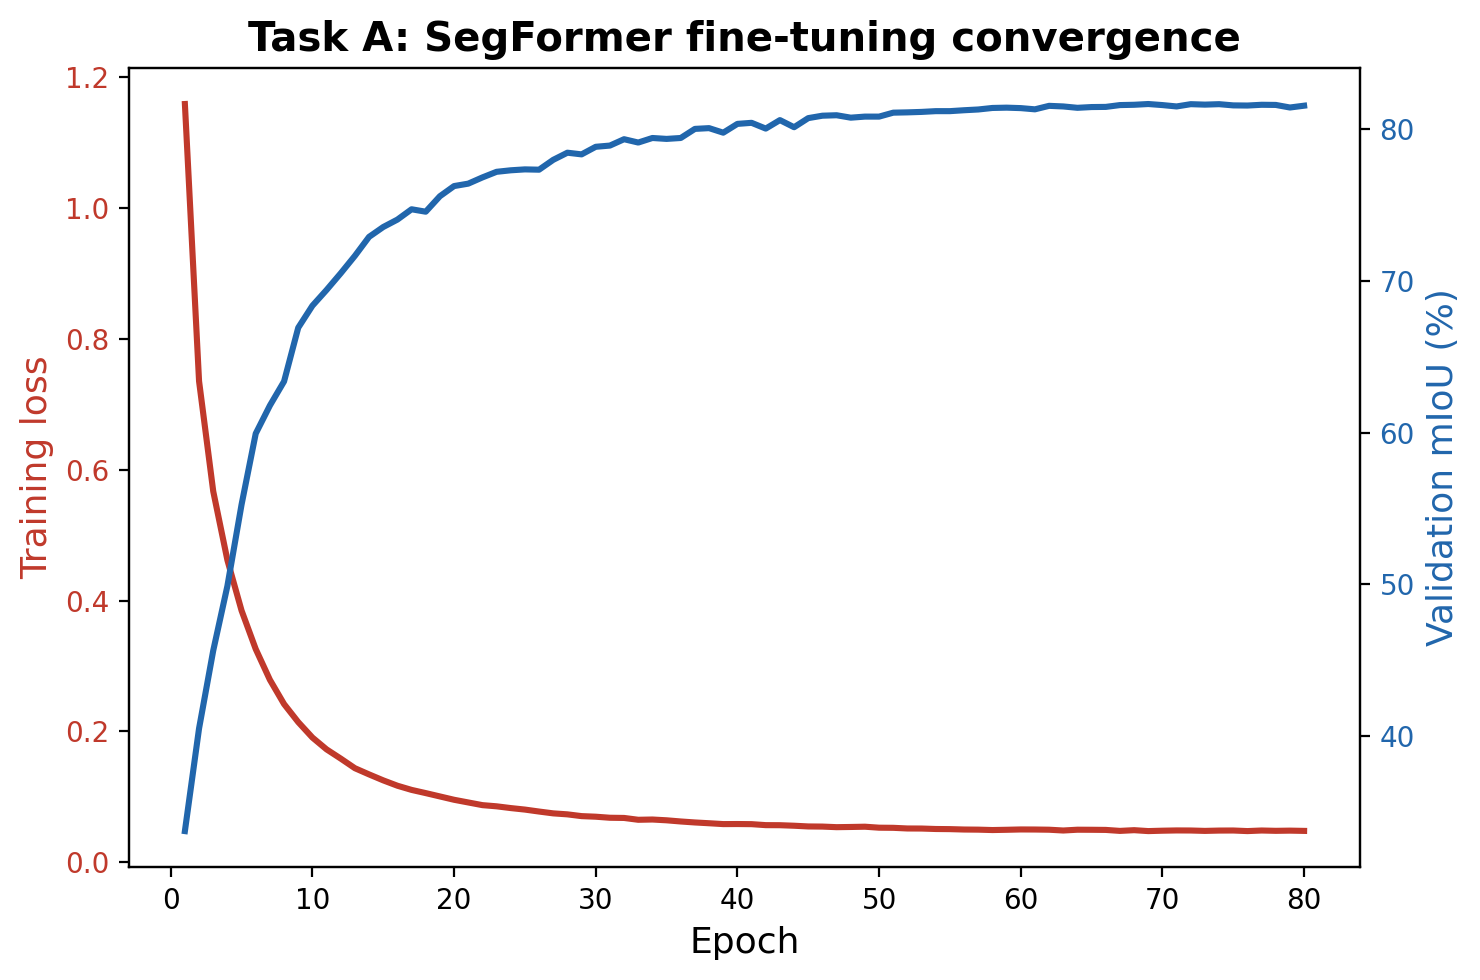
\includegraphics[width=\textwidth,height=.61\textheight,keepaspectratio]{fig9_task_a_training.png}\end{columns}
\begin{alertblock}{Metric boundary}Task A uses its 30-image internal validation split. These values are not Task B test results.\end{alertblock}
\source{DRAFT.md Table 1, Figure 9, and Section 4.2.}
\end{frame}

\begin{frame}{Semantic Gaussian representation}
\vspace{.45cm}
\[
g_k=\{\mu_k,s_k,q_k,o_k,c_k,\ell_k\},
\qquad c_k\in(0,1)^3,\quad \ell_k\in\mathbb R^5.
\]
\begin{itemize}\tightitems
\item $\mu_k$ and $s_k$ describe position and scale; $q_k$ is a unit rotation quaternion and $o_k$ is opacity.
\item Geometry, opacity, RGB, and semantic logits remain jointly trainable; RGB is view-independent.
\item Position and observed RGB originate from one sparse point, while multi-view votes initialize $\ell_k$.
\end{itemize}
\begin{block}{Eight trainable rendering channels}
The renderer concatenates three RGB values $c_k$ and five class logits $\ell_k$ for each Gaussian.
\end{block}
\source{DRAFT.md Section 3.4.}
\end{frame}

\begin{frame}{Semantic Gaussian architecture}
\begin{center}
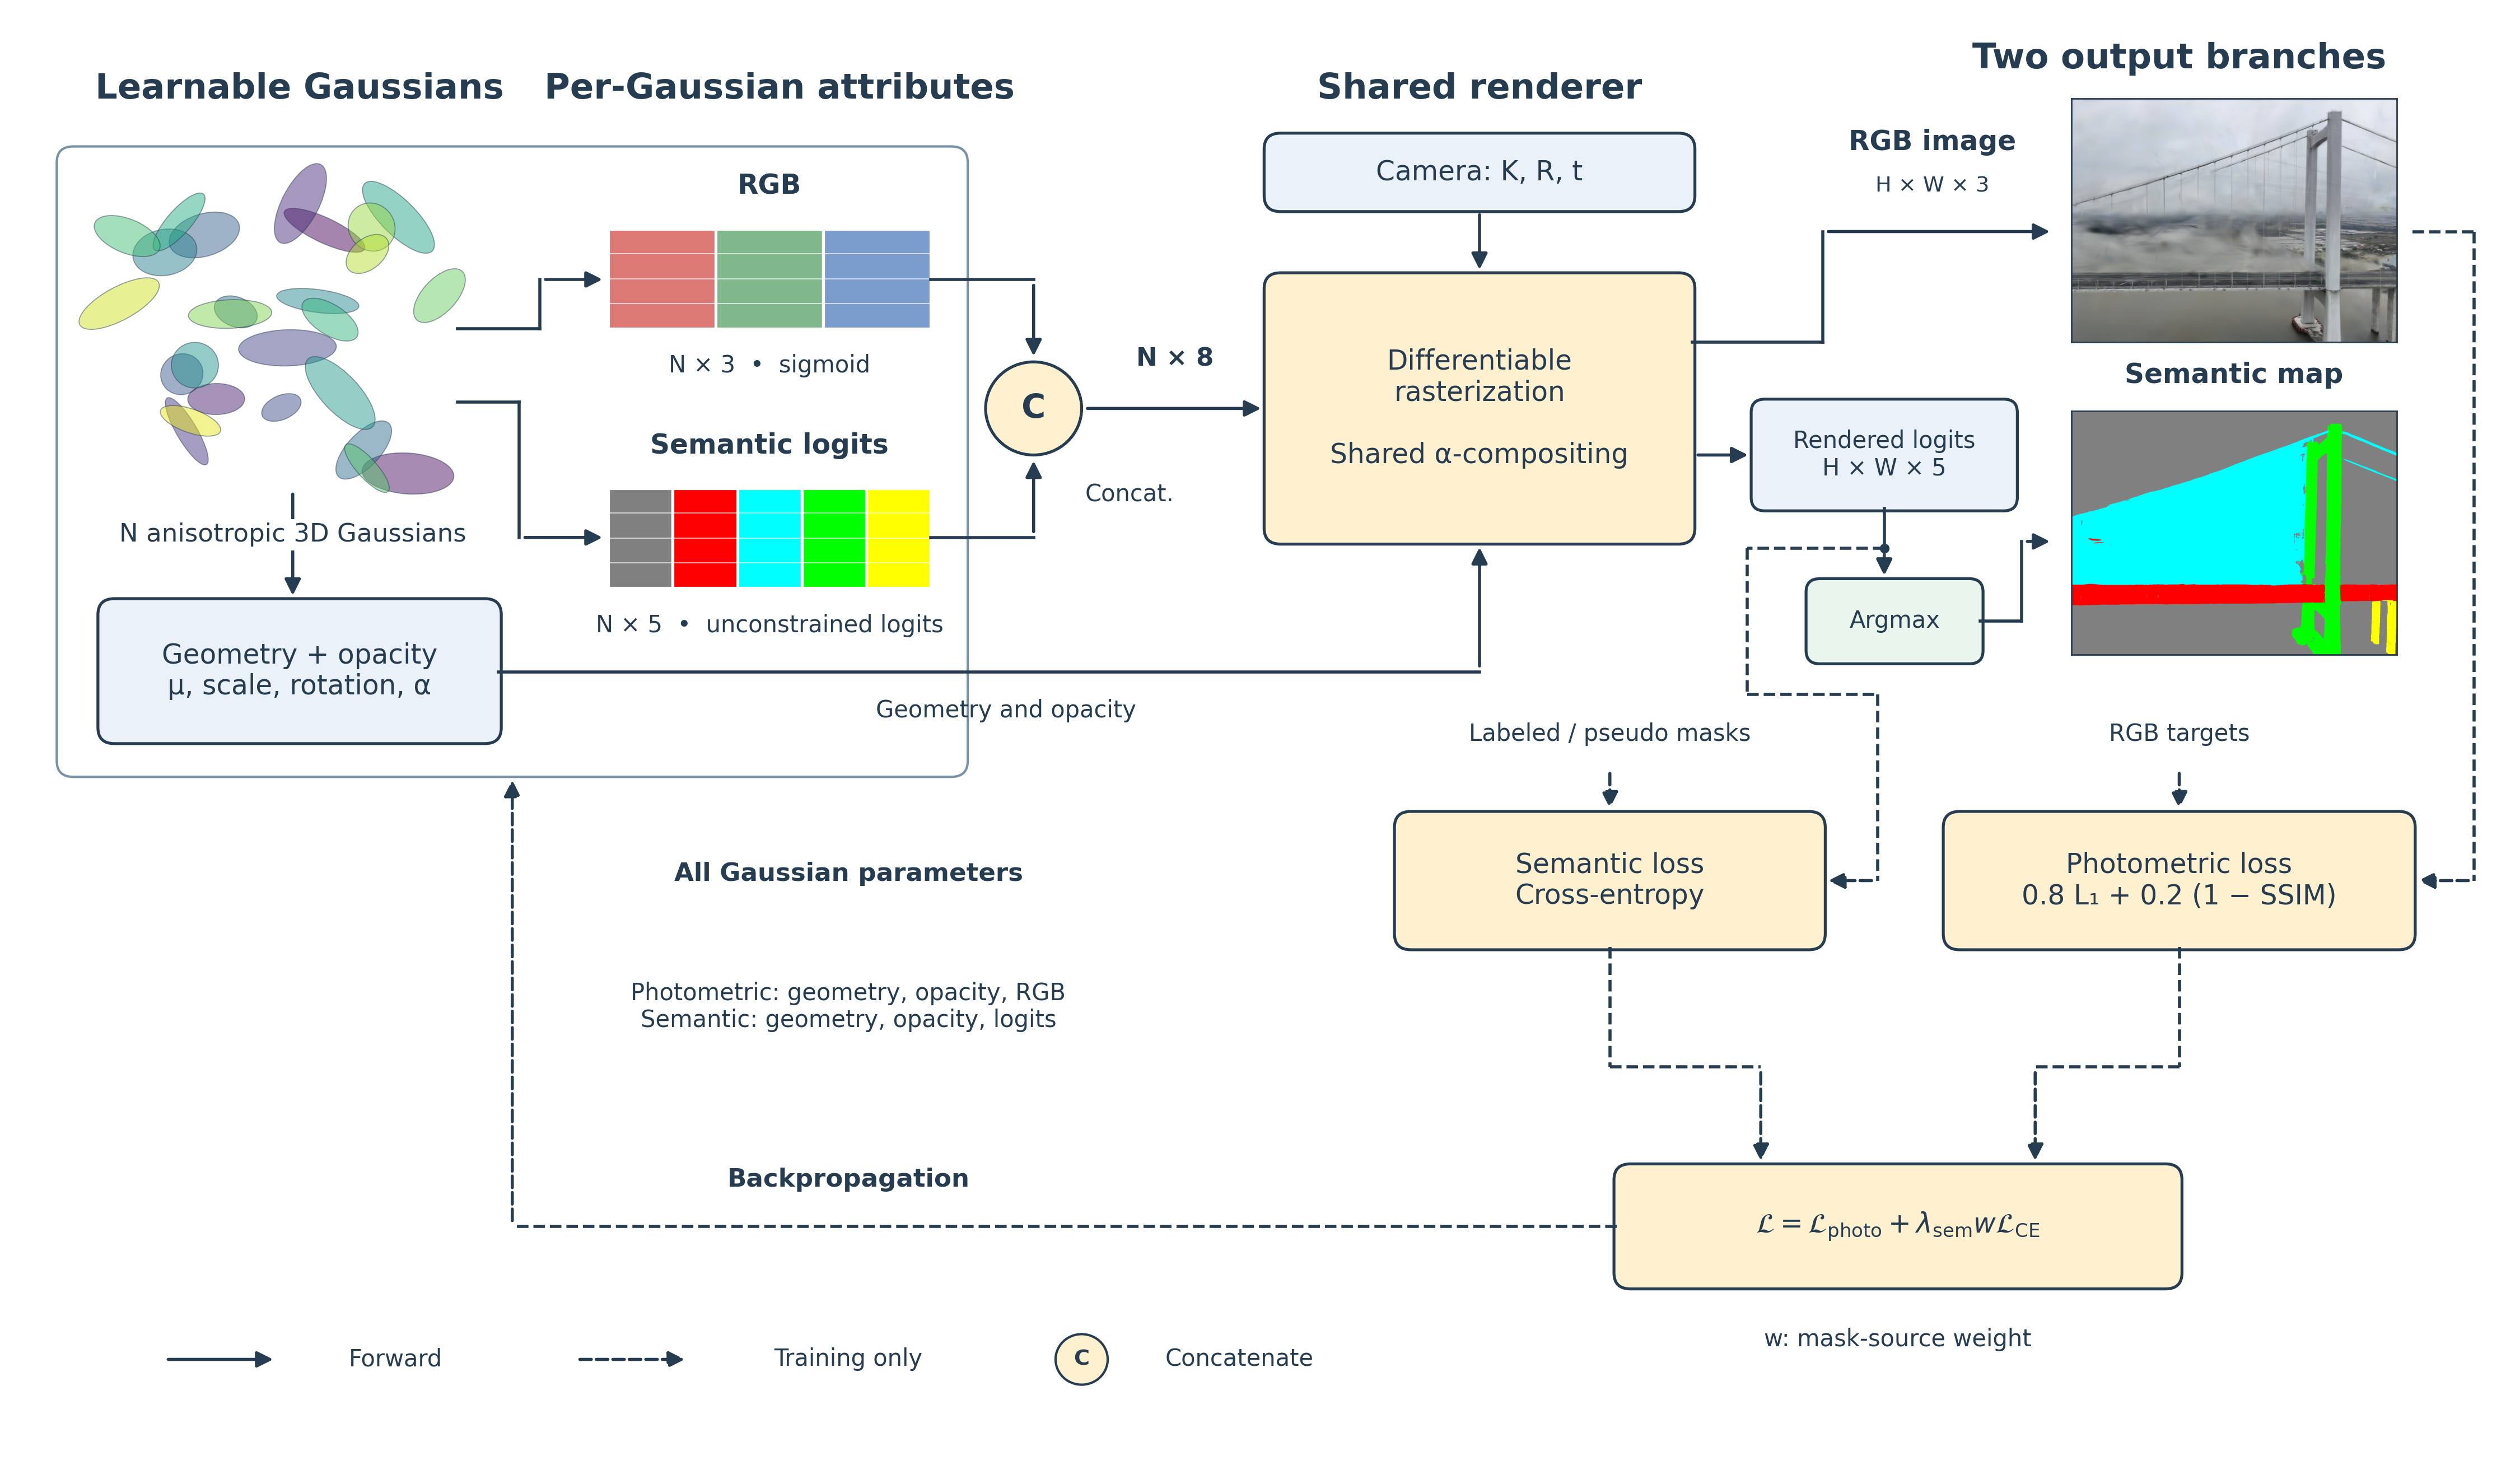
\includegraphics[width=1.02\textwidth,height=.84\textheight,keepaspectratio]{fig4_gaussian_architecture.png}
\end{center}
\source{DRAFT.md Section 3.4 and Figure 4.}
\end{frame}

\begin{frame}{Semantic warm-start}
\begin{center}
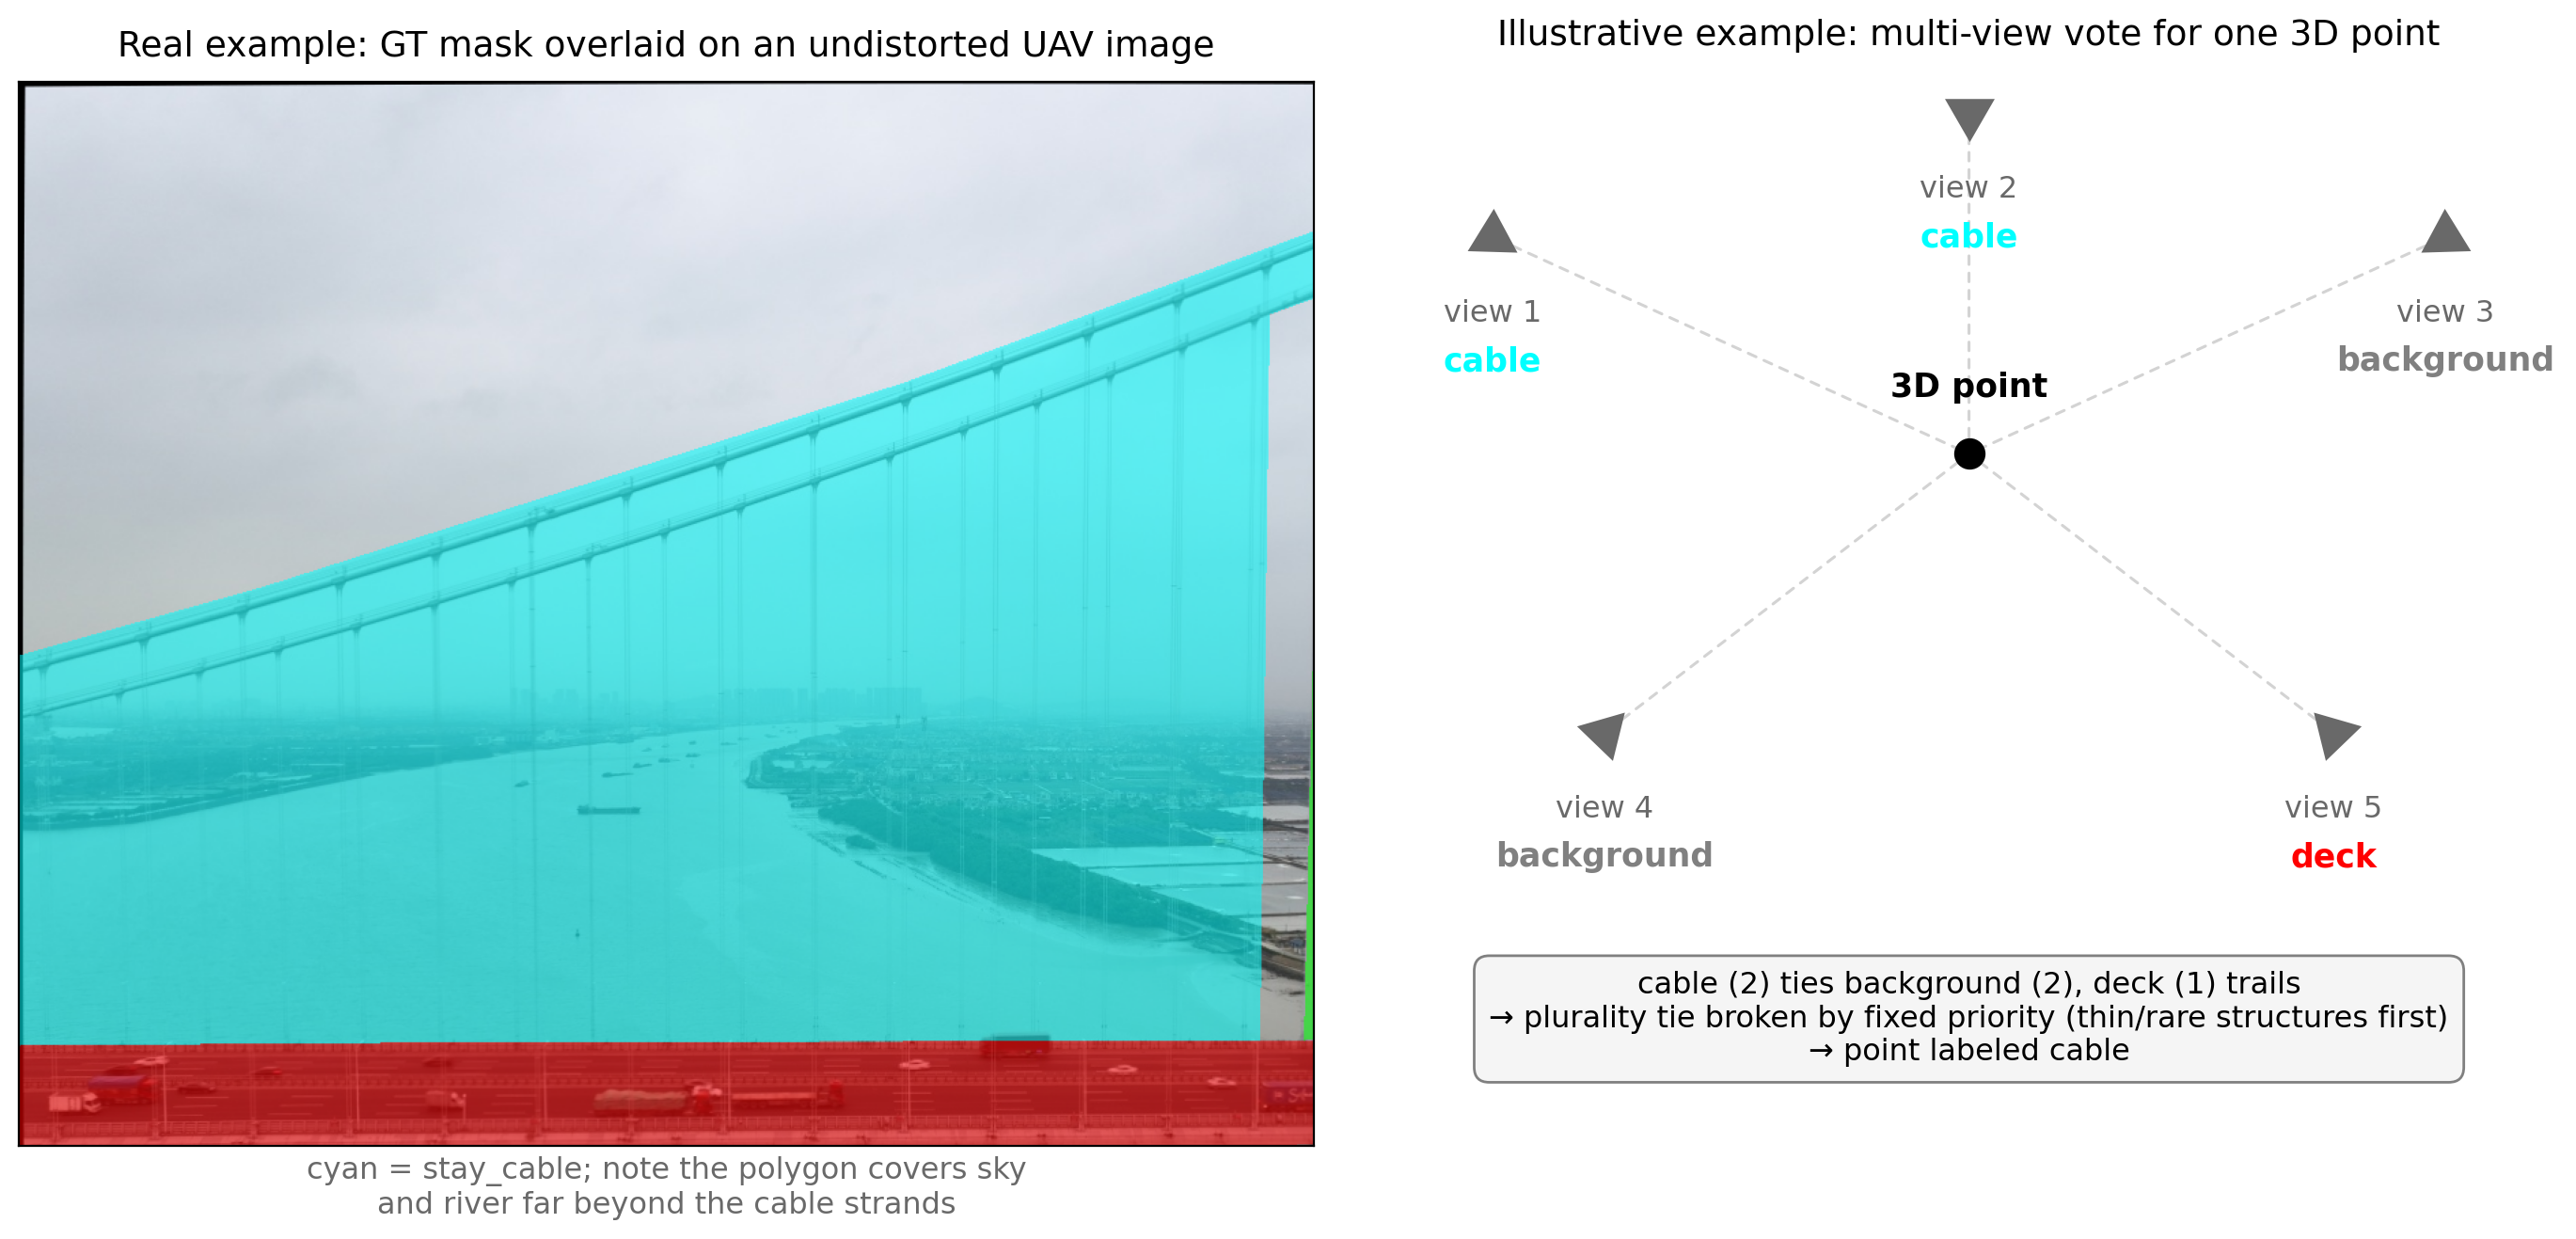
\includegraphics[width=.93\textwidth,height=.56\textheight,keepaspectratio]{fig3_cable_voting.png}
\end{center}
\vspace{-.3em}
\begin{itemize}\tightitems
\item Each labeled observation votes at its track coordinate. The plurality winner initializes $+2$ for its class and $-2$ for the others.
\item Ties use the priority cable, tower, foundation, deck, background. Pseudo-labels supervise training but do not vote during initialization.
\item The broad cable polygon defines the semantic target; it does not resolve individual strands.
\end{itemize}
\source{DRAFT.md Section 3.4 and Figure 3.}
\end{frame}

\begin{frame}{Fused RGB and semantic rendering}
\small
\[T_{kp}=\prod_{j<k}(1-a_{jp}),\qquad T_{\mathrm{end},p}=\prod_k(1-a_{kp}).\]
\[\hat I_p=\sum_kT_{kp}a_{kp}c_k+T_{\mathrm{end},p}b_I,\qquad z_p=\sum_kT_{kp}a_{kp}\ell_k+T_{\mathrm{end},p}b_\ell.\]
\[\hat M_p=\arg\max_cz_{pc},\qquad b_I=(.5,.5,.5),\quad b_\ell=(4,-4,-4,-4,-4).\]
\begin{block}{Implementation consequence}Three RGB channels and five logits form one eight-channel gsplat pass \textup{[7]}. Both outputs share projection, visibility, depth order, and alpha-compositing weights.\end{block}
\source{DRAFT.md Section 3.4; gsplat.}
\end{frame}

\begin{frame}{Joint optimization objective}
\small
\[\frac{\partial\mathcal L_{\mathrm{CE},p}}{\partial\ell_k}=T_{kp}a_{kp}\bigl(\operatorname{softmax}(z_p)-e_{y_p}\bigr).\]
\[\mathcal L=\mathcal L_{\mathrm{photo}}+\lambda_{\mathrm{sem}}\omega\mathcal L_{\mathrm{sem}},\qquad\mathcal L_{\mathrm{photo}}=.8\mathcal L_1+.2(1-\mathrm{SSIM}).\]
\[\lambda_{\mathrm{sem}}=.5,\qquad\omega=\begin{cases}1&\text{manual annotation},\\.5&\text{pseudo-label}.\end{cases}\]
\begin{itemize}\tightitems
\item Semantic loss updates logits and shared geometry/opacity through compositing weights.
\item Photometric loss directly updates RGB, geometry, and opacity, with no direct gradient to logits.
\end{itemize}
\source{DRAFT.md Section 3.4.}
\end{frame}

\begin{frame}{Mask alignment and observed-color initialization}
\begin{columns}[T,onlytextwidth]\column{.49\textwidth}
\textbf{Coordinate alignment}
\begin{itemize}\tightitems
\item Polygons and SegFormer predictions originate in distorted photographs.
\item Task B renders undistorted pinhole images.
\item Images and masks receive the same remap; masks use nearest-neighbor interpolation.
\item Voting remains in original coordinates because COLMAP tracks reference original images.
\end{itemize}
\column{.49\textwidth}
\textbf{Appearance initialization}
\begin{itemize}\tightitems
\item Sample each point's RGB at every retained non-test observation.
\item Average observations to initialize one Gaussian's color.
\item Unlabeled views may contribute RGB; test views remain excluded.
\item Scales use three-neighbor distance; rotation starts at identity and opacity at 0.3.
\end{itemize}\end{columns}
\source{DRAFT.md Sections 3.2 and 3.4.}
\end{frame}

\begin{frame}{Task B experimental setup}
\begin{columns}[T,onlytextwidth]\column{.55\textwidth}\begin{itemize}\tightitems
\item 370 supervised views: 270 manual masks and 100 pseudo-masks.
\item 40,000 iterations at $1320\times989$; seed 42.
\item Adam rates: means $1.6\times10^{-4}$, scales $5\times10^{-3}$, rotation $10^{-3}$, opacity $5\times10^{-2}$, RGB/logits $2.5\times10^{-3}$.
\item Density control every 100 steps from 500 to 15,000; 600,000-Gaussian soft cap.
\end{itemize}
\column{.42\textwidth}
\begin{block}{Representation growth}82,518 initial points\\600,583 final Gaussians\\stable after step 7,400\end{block}
\begin{block}{Compute}NVIDIA RTX 3080 (10 GB)\\about 46 minutes at full resolution\end{block}\end{columns}
\source{DRAFT.md Sections 4.1 and 4.2.}
\end{frame}

\section{Results}
\begin{frame}{Task B aggregate test results}
\begin{columns}[T,onlytextwidth]\column{.47\textwidth}
\begin{tabular}{lr}\toprule Metric&Value\\\midrule PSNR&22.43 dB\\SSIM&0.854\\LPIPS&0.321\\Structural mIoU&\textbf{92.08\%}\\Five-class mIoU&93.5\%\\Illustrative Accuracy Score&0.823\\\bottomrule\end{tabular}
\column{.50\textwidth}\begin{itemize}\tightitems
\item Metrics use 30 held-out, undistorted views.
\item Structural mIoU averages four bridge classes equally; background is excluded.
\item The illustrative Accuracy Score is our interpretation of the brief, not a blind-test score.
\item The split evaluates interpolation near the released trajectory with supplied geometry.
\end{itemize}\end{columns}
\source{DRAFT.md Table 2 and Section 3.6.}
\end{frame}

\begin{frame}{Task B per-class semantic results}
\begin{columns}[T,onlytextwidth]\column{.61\textwidth}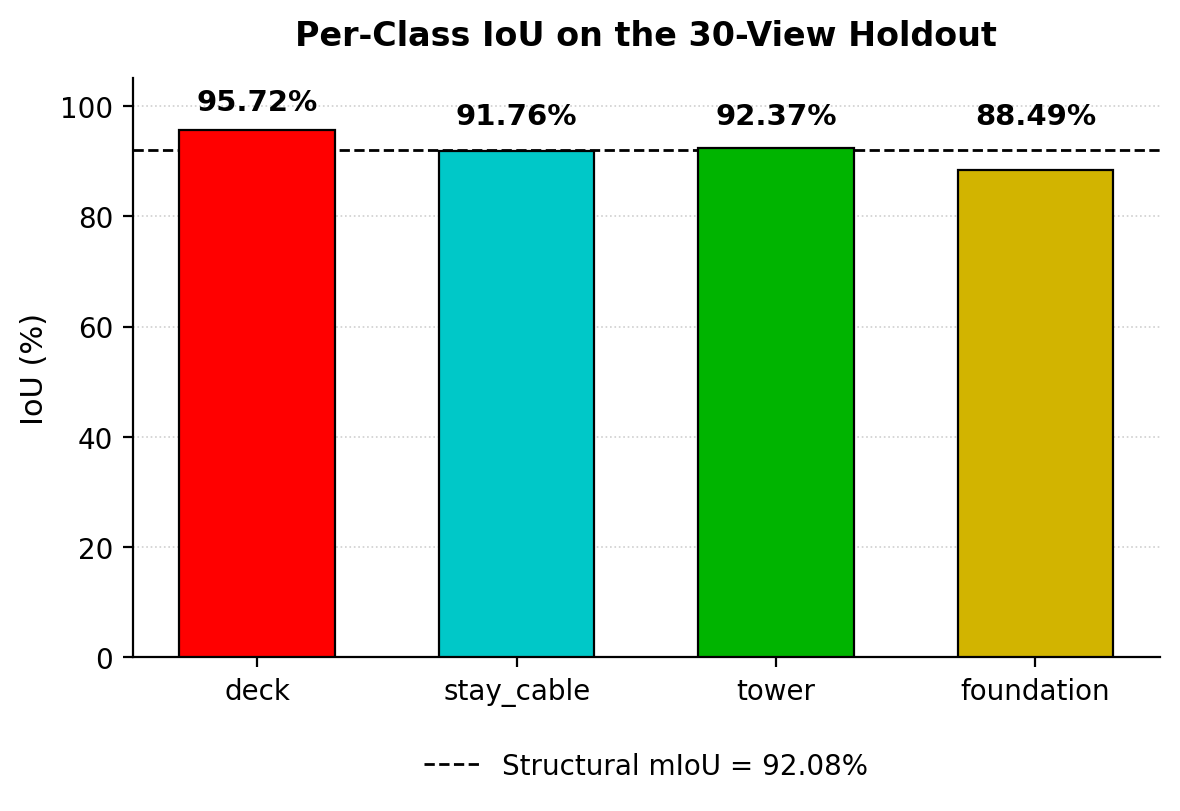
\includegraphics[width=\textwidth,height=.67\textheight,keepaspectratio]{fig5_per_class_iou.png}
\column{.36\textwidth}\begin{itemize}\tightitems
\item Deck: 95.72\%.
\item Tower: 92.37\%.
\item Stay cable: 91.76\%.
\item Foundation: 88.49\%.
\item Background: 99.20\%, reported separately.
\end{itemize}
\end{columns}
\source{DRAFT.md Table 3, Figure 5, and Section 5.2.}
\end{frame}

\begin{frame}{Qualitative held-out views}
\begin{center}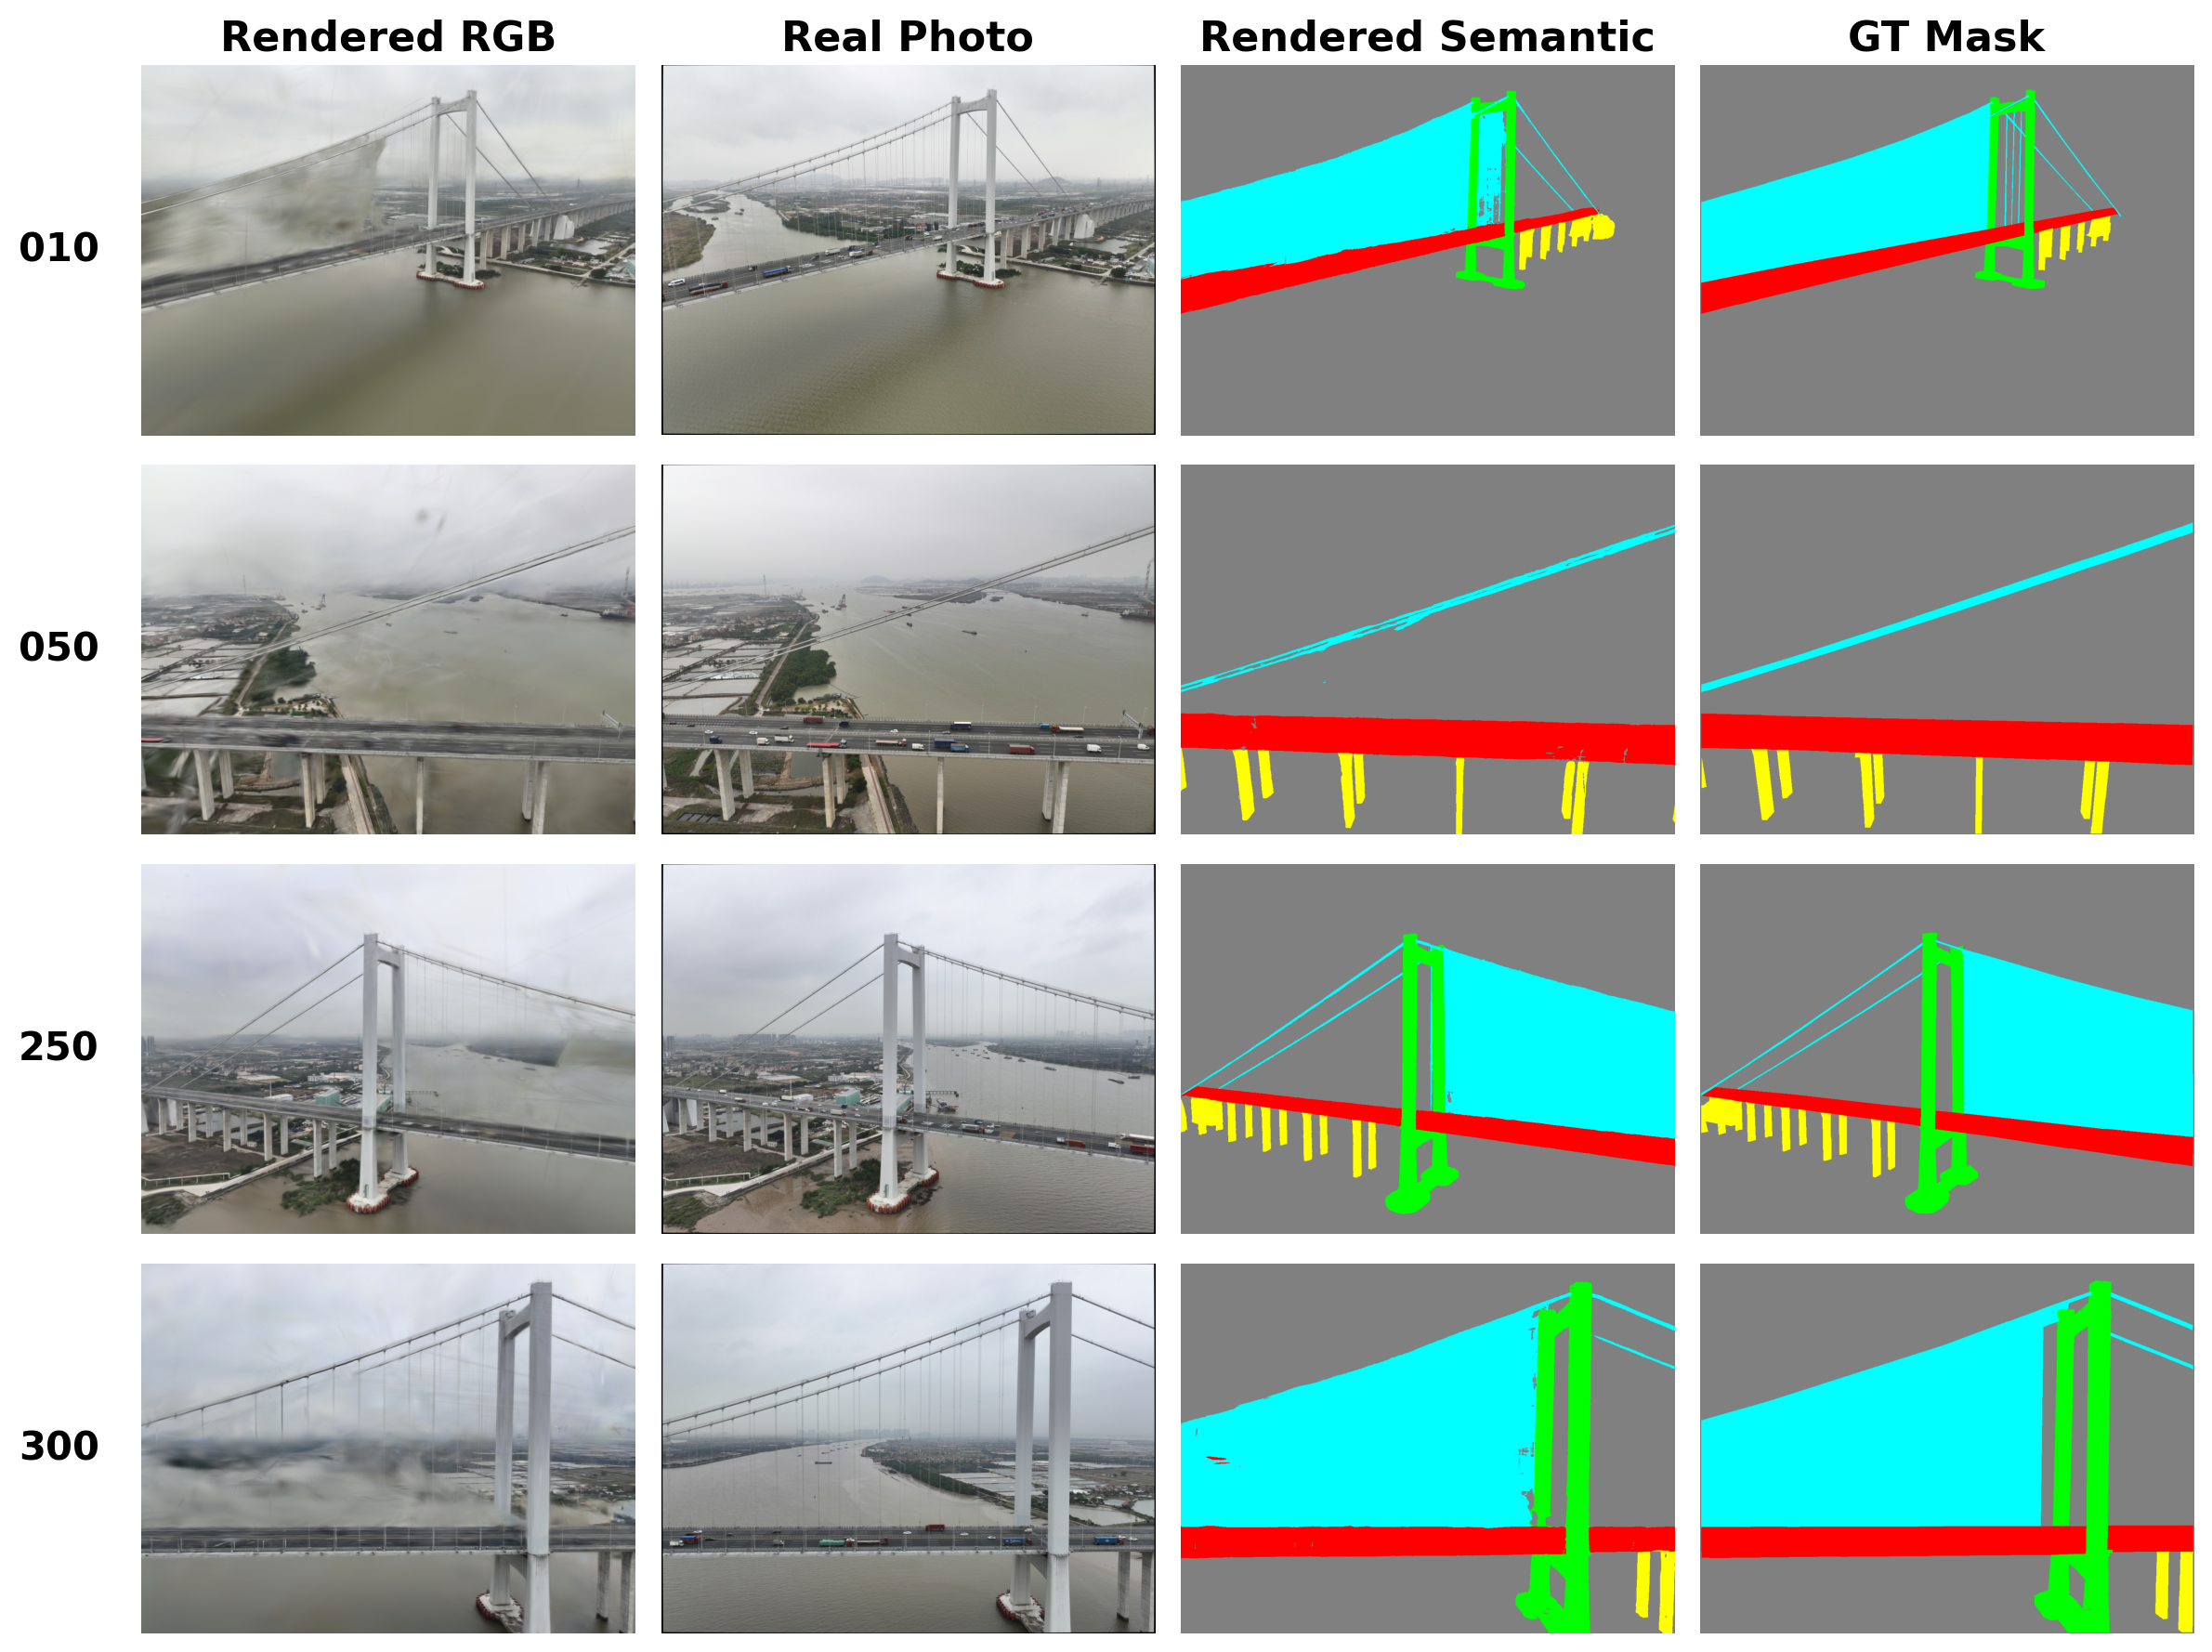
\includegraphics[width=.90\textwidth,height=.61\textheight,keepaspectratio]{fig6_qualitative_grid.png}\end{center}
\vspace{-.3em}\begin{itemize}\tightitems
\item View 250 is the cleanest RGB example; views 010 and 300 show visible blur and streaking.
\item Semantic regions remain recognizable despite appearance artifacts, but four examples do not replace full-holdout statistics.
\end{itemize}
\source{DRAFT.md Figure 6 and Section 5.3.}
\end{frame}

\begin{frame}{Rendering between observed viewpoints}
\begin{center}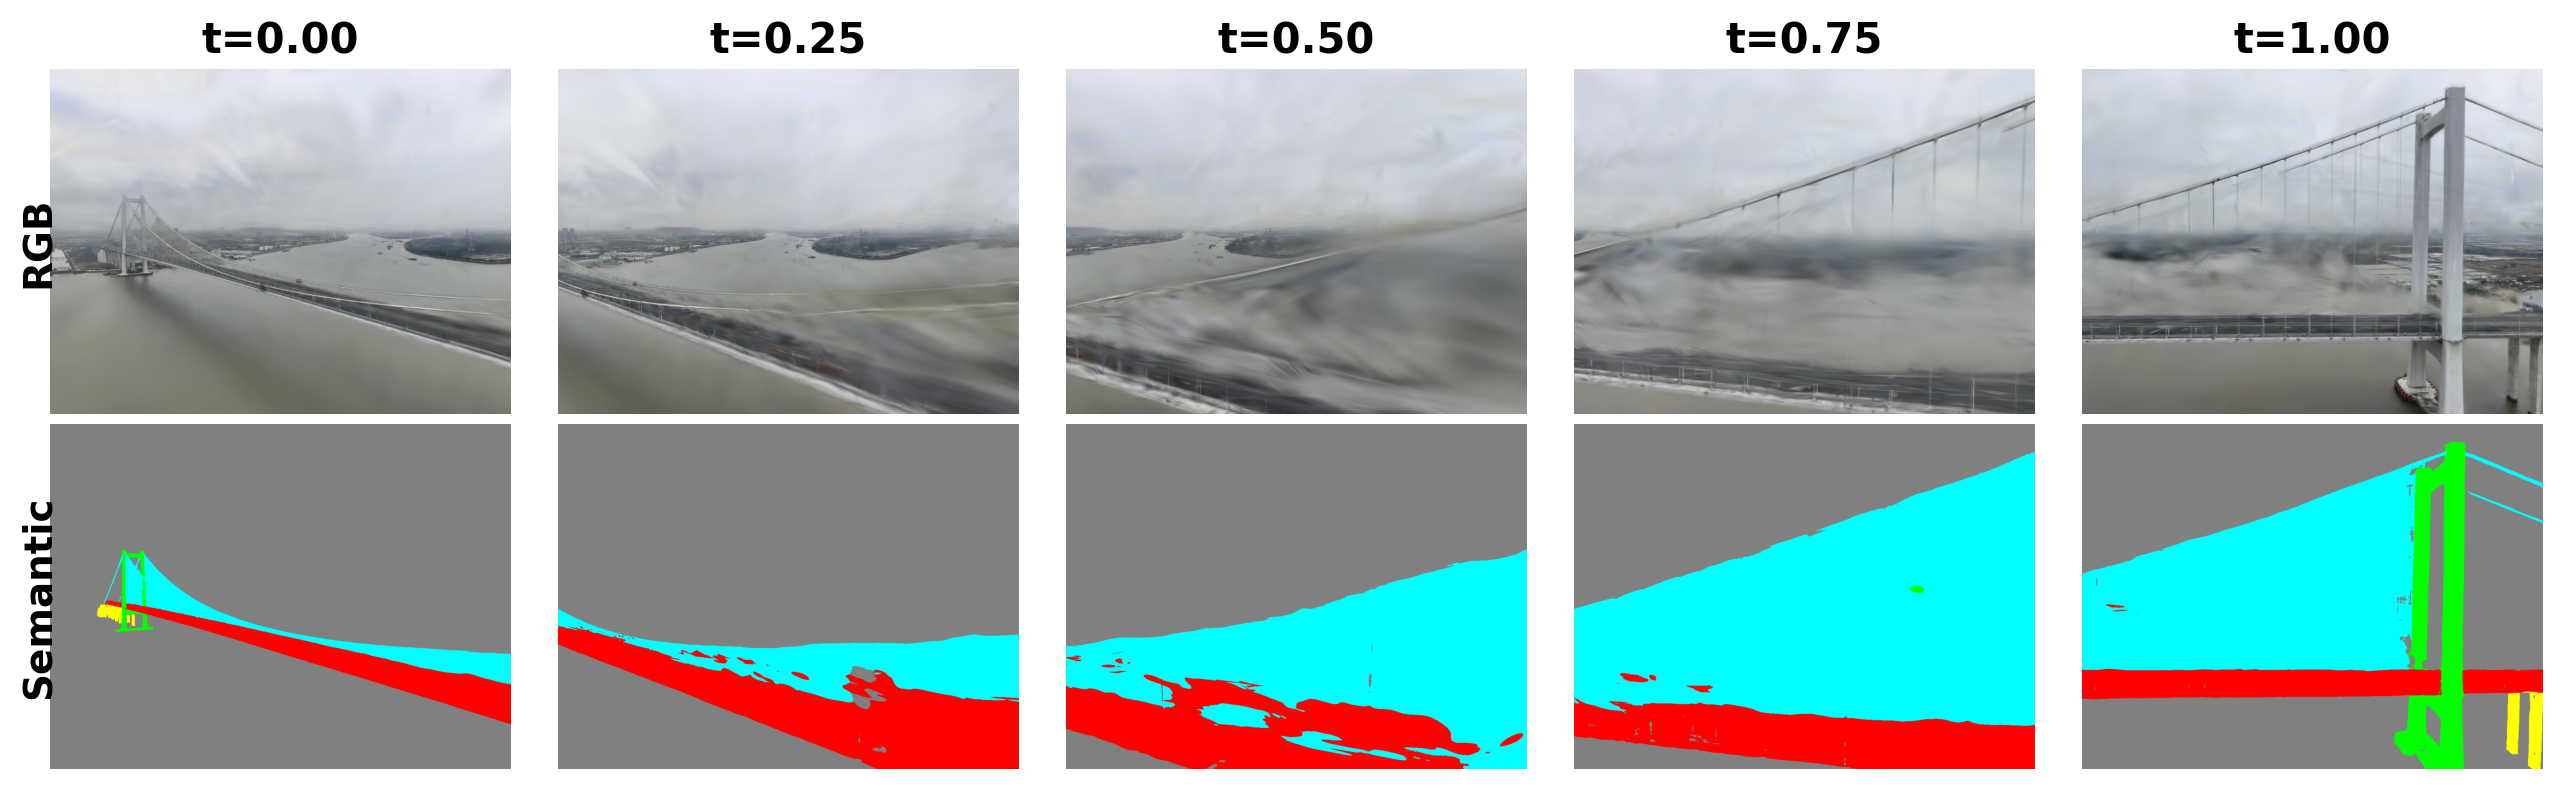
\includegraphics[width=.90\textwidth,height=.59\textheight,keepaspectratio]{fig7_interpolation.png}\end{center}
\vspace{-.3em}\begin{itemize}\tightitems
\item Rotation uses quaternion SLERP; translation interpolates world-to-camera translation between test poses 280 and 300.
\item Intermediate poses have no ground-truth photographs and provide a qualitative interface demonstration only.
\item RGB blur and semantic holes increase along parts of the path. Shared rasterization preserves alignment, not correctness.
\end{itemize}
\source{DRAFT.md Figure 7 and Section 5.3.}
\end{frame}

\begin{frame}{Explicit RGB and semantic splats}
\begin{center}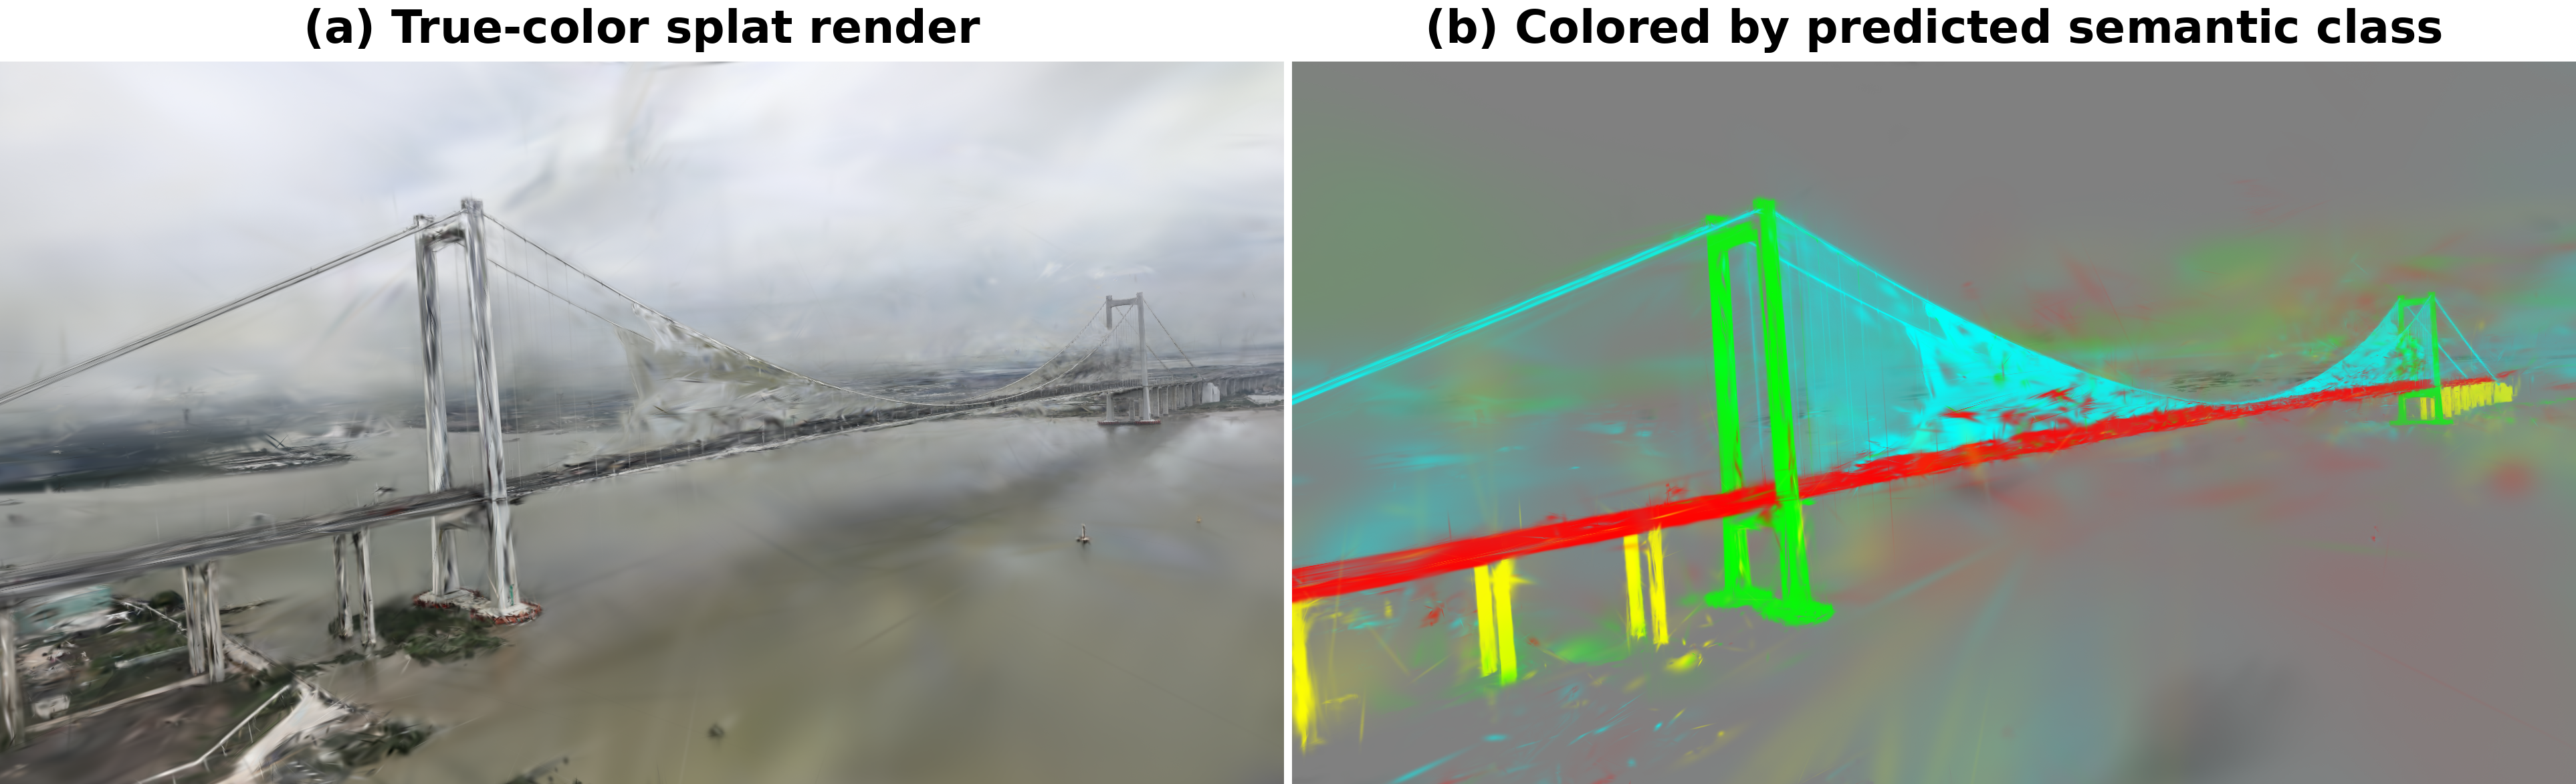
\includegraphics[width=.90\textwidth,height=.67\textheight,keepaspectratio]{fig8_splat_render.png}\end{center}
\vspace{-.2em}\begin{itemize}\tightitems
\item One trained representation appears as learned RGB and per-Gaussian argmax class colors.
\item Both screenshots use the same viewer camera pose, enabling direct spatial comparison of RGB appearance and per-Gaussian semantic colors.
\item Per-Gaussian recoloring differs from evaluated semantic rendering, which composites logits before argmax.
\end{itemize}
\source{DRAFT.md Figure 8 and Section 5.3.}
\end{frame}

\begin{frame}{Training convergence}
\begin{columns}[T,onlytextwidth]\column{.48\textwidth}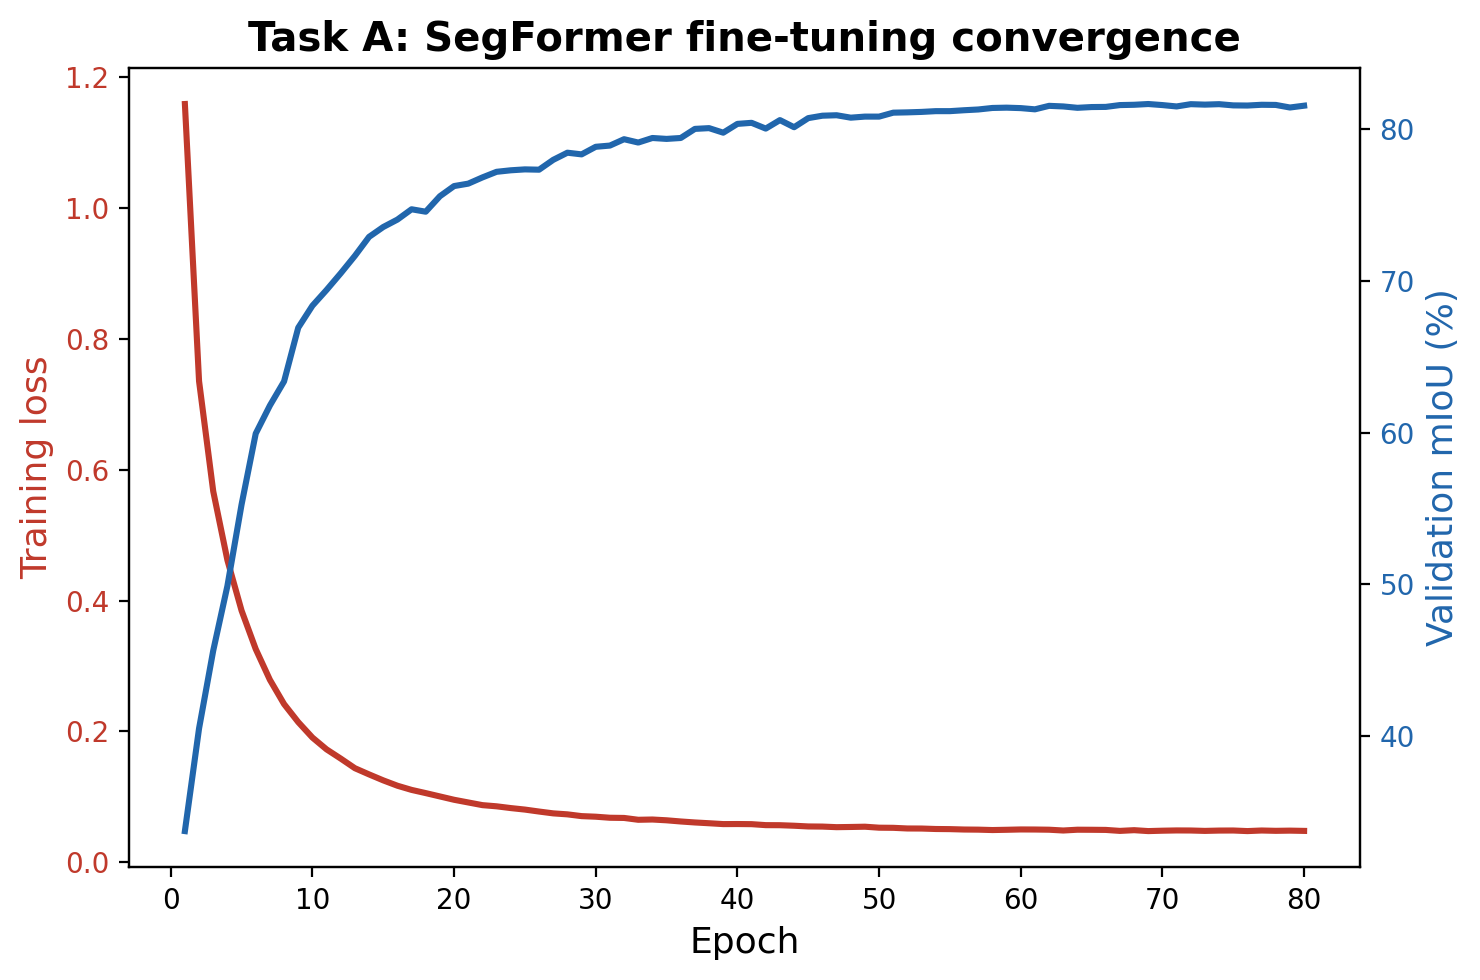
\includegraphics[width=\textwidth,height=.53\textheight,keepaspectratio]{fig9_task_a_training.png}\par\centering\tiny Task A: best validation mIoU 81.67\% at epoch 69.
\column{.48\textwidth}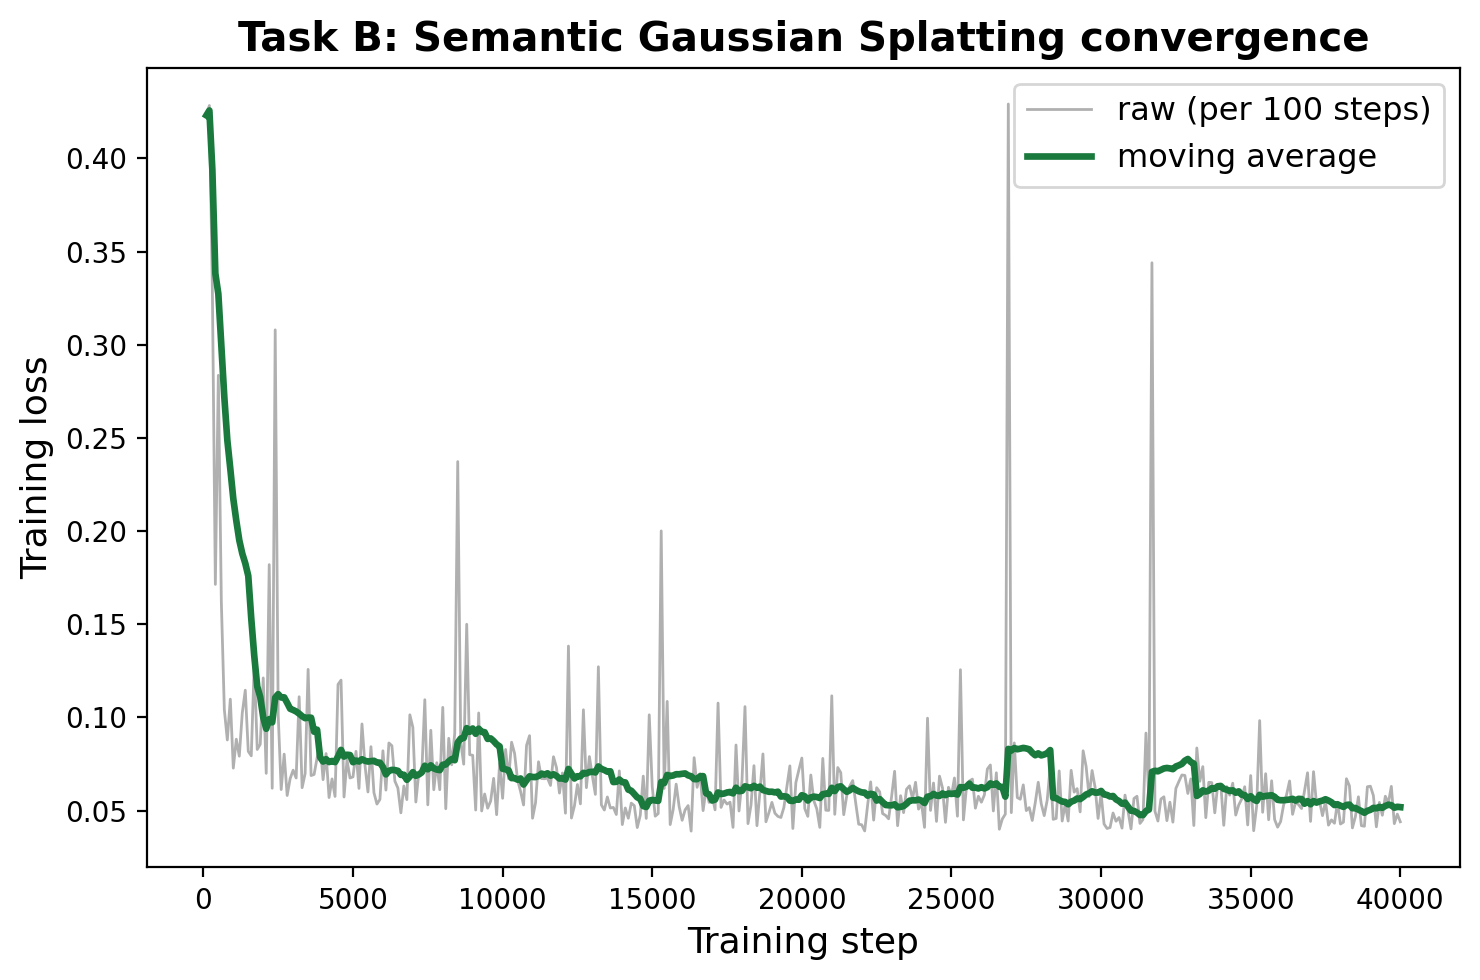
\includegraphics[width=\textwidth,height=.53\textheight,keepaspectratio]{fig10_task_b_training.png}\par\centering\tiny Task B: sampled-view loss and moving average.\end{columns}
\vspace{.25em}\begin{itemize}\tightitems
\item Task A curves summarize epoch averages; Task B logs one sampled view every 100 steps.
\item Their loss scales are not comparable. Final Task B performance is measured on the test split.
\end{itemize}
\source{DRAFT.md Figures 9--10 and Section 5.4.}
\end{frame}

\begin{frame}{Resolution ablation}
\begin{center}
\begin{tabular}{lrrrr}\toprule Training&PSNR&SSIM&LPIPS&$\structmiou$\\\midrule Half&22.03&.838&.330&89.71\%\\\textbf{Full}&\textbf{22.43}&\textbf{.854}&\textbf{.321}&\textbf{92.08\%}\\\bottomrule\end{tabular}
\end{center}
\vspace{.5em}\begin{itemize}\tightitems
\item Matched 40,000-step runs share the split, poses, initialization, losses, density schedule, and full-resolution evaluation.
\item Full resolution improves PSNR by 0.40 dB, SSIM by 0.016, and structural mIoU by 2.37 points; LPIPS decreases by 0.009.
\item Training time increases from about 18 to 46 minutes on the same RTX 3080.
\item One run per resolution does not quantify random-seed uncertainty.
\end{itemize}
\source{DRAFT.md Table 4 and Section 5.5.}
\end{frame}

\section{Discussion}
\begin{frame}{What the evaluation establishes}
\begin{itemize}\tightitems
\item One explicit Gaussian scene renders aligned RGB and five-class semantic outputs.
\item On 30 local test views, the final model reaches 22.43 dB PSNR and 92.08\% structural mIoU.
\item Test observations are excluded from losses, voting, triangulation, and color initialization.
\item The interleaved split samples viewpoints near training frames and mainly tests interpolation under supplied geometry.
\item Full-resolution training outperforms the matched half-resolution run within the tested budget.
\end{itemize}
\begin{alertblock}{Claim boundary}The results establish agreement with released images and masks near the flight trajectory, not unrestricted viewpoint generalization or metric 3D accuracy.\end{alertblock}
\source{DRAFT.md Sections 3.6 and 5.}
\end{frame}

\begin{frame}{Limitations}
\begin{itemize}\tightitems
\item The interleaved holdout does not test a spatially separated trajectory segment.
\item Supplied poses and calibration originate from the released collection; sensitivity to independent pose estimation is unknown.
\item Coarse cable polygons cannot validate individual strand geometry or boundaries.
\item Constructed novel poses show artifacts in both RGB and semantics and have no ground truth.
\item The system has not been evaluated for damage detection, deformation, cable force, or structural response.
\end{itemize}
\source{DRAFT.md Sections 5.3--6.}
\end{frame}

\begin{frame}{Conclusion}
\begin{itemize}\tightitems
\item SegFormer expands semantic supervision from 270 manually labeled views to 370 views.
\item Sparse geometry, observed colors, and plurality votes initialize an explicit semantic Gaussian scene.
\item One differentiable rasterization pass produces aligned RGB and five semantic-logit channels.
\item Local test performance is 22.43 dB PSNR, 0.854 SSIM, 0.321 LPIPS, and 92.08\% structural mIoU.
\item Full-resolution training improves every reported metric relative to the matched half-resolution run.
\item Future tests should use spatially separated views, independent geometry, and finer cable annotations.
\end{itemize}
\begin{block}{Outcome}A renderable, component-labeled bridge representation with explicit limits on geometric and out-of-trajectory claims.\end{block}
\end{frame}

\begin{frame}{Selected references}
\scriptsize\begin{enumerate}\tightitems
\item IC-SHM 2026 Organizing Committee, ``The 4th International Project Competition for Structural Health Monitoring,'' Project 2 competition brief, pp. 9--10, 2026.
\item J. L. Sch\"onberger and J.-M. Frahm, ``Structure-from-Motion Revisited,'' CVPR, 2016.
\item B. Kerbl et al., ``3D Gaussian Splatting for Real-Time Radiance Field Rendering,'' ACM Transactions on Graphics, 42(4), Article 139, 2023.
\item S. Zhi et al., ``In-Place Scene Labelling and Understanding with Implicit Scene Representation,'' ICCV, 2021.
\item S. Zhou et al., ``Feature 3DGS: Supercharging 3D Gaussian Splatting to Enable Distilled Feature Fields,'' CVPR, 2024.
\item E. Xie et al., ``SegFormer: Simple and Efficient Design for Semantic Segmentation with Transformers,'' NeurIPS, 2021.
\item V. Ye et al., ``gsplat: An Open-Source Library for Gaussian Splatting,'' Journal of Machine Learning Research, 26(34), 1--17, 2025.
\end{enumerate}
\end{frame}
\end{document}
